\section{Method}
\subsection{Objective function and gradients of elastic WERTI}
Assume that there is a perturbation $\delta c_{ijkl}$ in the background elastic media
$c_{ijkl}$, the background wavefileds $u_i$ and perturbed wavefields
$\delta u_i$ satisfy:
\begin{equation}
    \rho \frac{\partial u^2_i}{\partial t^2}  -
    \frac{\partial}{\partial x_j}\left[ 
        c_{ijkl}\frac{\partial u_{k}}{\partial
        x_l}\right]=f_i,
    \label{eq:WE} 
\end{equation}
and
\begin{equation}
    \rho \frac{\partial \delta u^2_i}{\partial t^2}  -
    \frac{\partial}{\partial x_j}\left[ 
        c_{ijkl}\frac{\partial \delta u_{k}}{\partial
        x_l}\right]=\frac{\partial}{\partial x_j}\left[\delta c_{ijkl}\frac{\partial u_{k}}{\partial x_l}\right],
    \label{eq:DeltaWE} 
\end{equation}
where $\delta u_i$ can be seen as the demigrated reflection data using the image
perturbation $\delta c_{ijkl}$ obtained from RTM or other imaging method. In WERTI, we
aim to minimize the traveltime differences between observed data
$\mathbf{d}^{o}$ and
calculated data $\mathbf{d}^{c}$, then
the objective function is:
%\begin{equation}
%	E=\frac{1}{2}\int\tau^2(\mathbf{x_r},t;\mathbf{x_s})dtd\mathbf{x_r}d\mathbf{x_s},
%    \label{eq:Objectivefunction} 
%\end{equation}
\begin{equation}
	\left\{
		\begin{aligned}
			&\tau(\mathbf{x_r},t;\mathbf{x_s})=\mathop{\arg\min}_{\tau}
			\parallel\mathbf{d}^{c}(\mathbf{x}_r,t;\mathbf{x}_s)-\mathbf{d}^{o}(\mathbf{x}_r,t+\tau;\mathbf{x}_s)\parallel^2\\
    &E=\frac{1}{2}\int\tau^2(\mathbf{x_r},t;\mathbf{x_s})dtd\mathbf{x_r}d\mathbf{x_s},
		\end{aligned}
	\right.
    \label{eq:Objectivefunction} 
\end{equation}
where the time differences $\tau(\mathbf{x_r},t;\mathbf{x_s})$ can be extracted
through DIW.
After a similar derivation as in \cite{Ma2013}, the gradients of equation \eqref{eq:Objectivefunction} can be expressed as:
\begin{equation}
	\frac{\partial E}{\partial c_{ijkl}}=-\int (\frac{\partial u_{i}}{\partial
	x_j}\frac{\partial \delta \psi_{k}}{\partial x_l}+\frac{\partial \delta u_{i}}{\partial
	x_j}\frac{\partial \psi_{k}}{\partial x_l}),
    \label{eq:GradientCijkl}
\end{equation}
where $\psi_i$ and $\delta \psi_i$ are the adjoint wavefields satisfying:
\begin{equation}
    \rho \frac{\partial \psi^2_i}{\partial t^2}  -
    \frac{\partial}{\partial x_j}\left[ 
        c_{ijkl}\frac{\partial \psi_{k}}{\partial
		x_l}\right]=\tau(\mathbf{x_r},t;\mathbf{x_s})\frac{\dot{d}^o_i(\mathbf{x_r},t+\tau;\mathbf{x_s})}{h_i(\mathbf{x_r},t;\mathbf{x_s})},
    \label{eq:AdjointWE} 
\end{equation}
and
\begin{equation}
    \rho \frac{\partial \delta \psi^2_i}{\partial t^2}  -
    \frac{\partial}{\partial x_j}\left[ 
        c_{ijkl}\frac{\partial \delta \psi_{k}}{\partial
        x_l}\right]=\frac{\partial}{\partial x_j}\left[\delta c_{ijkl}\frac{\partial
		\psi_{k}}{\partial x_l}\right],
    \label{eq:AdjointDeltaWE} 
\end{equation}
with
$h_i(\mathbf{x_r},t)=\dot{d}^o_i(\mathbf{x_r},t+\tau)^2-\ddot{d}^o_i(\mathbf{x_r},t+\tau)(d^c_i(\mathbf{x_r},t)-d^o_i(\mathbf{x_r},t+\tau)$. The
hat dot denotes the time derivative. On the right hand side (RHS) of equation
\eqref{eq:GradientCijkl}, the first and second term indicate the source and receiver
part of the reflection wavepath, respectively. Then we can get the gradients in terms of P- and
S- wave velocities through the chain rule:
\begin{equation}
	\begin{split}
	&\frac{\partial E}{\partial V_p}=2\rho V_p\frac{\partial E}{\partial
		c_{ijkl}}\delta_{ij}\delta_{kl}, \\
	&\frac{\partial E}{\partial V_s}=2\rho V_s\frac{\partial
	E}{\partial c_{ijkl}}(-2\delta_{ij}\delta_{kl}+\delta_{ik}\delta_{jl}+
	\delta_{il}\delta_{jk}).
	\end{split}
    \label{eq:GradientVel}
\end{equation}

\subsection{Elastic Born reflection kernel analysis}
The key point of reflection inversion is to calculate the reflection kernel. 
RWI and WERTI utilize different objective functions which only induce different types of adjoint
sources, but share similar reflection kernels.
%Different types of objective funtion only induce different types of adjoint sources.
Due to the complex mode conversions in elastic wavefields, wavepath of elastic reflections will 
be far more complicated than that in acoustic case.
Here, we decompose the origin kernel into four components which 
represent cross-correlation of different wave modes.

For simplicity, we rewrite \eqref{eq:GradientCijkl} as follow:
\begin{equation}
    \nabla E(
    \mathbf{m}_0)=-\int(
    \mathbf{u}\cdot\delta \boldsymbol{\psi}
    +\delta
    \mathbf{u}\cdot{\boldsymbol{\psi}})
    \label{eq:kernelgradient} 
\end{equation} 
with $\mathbf{u}$ and $\boldsymbol{\psi}$ are the forward and adjoint background wavefields,
$\delta\mathbf{u}$ and $\delta \boldsymbol{\psi}$ are the forward and adjoint perturbed wavefields.
The operator $\cdot$ denotes the cross correlation between two wavefields. 
Note that, equation \eqref{eq:kernelgradient} just schematically shows the manner of cross correlation. 
The detailed formulas should be derived according to the parameter $\mathbf{m}_0$ through chain rule, just as equation \eqref{eq:GradientVel}.
Considering mode decomposition, the above formula can be decomposed into four types with:
\begin{equation}
    K_{m_0}^{MN}     
    =-\int(\mathbf{u}^M\cdot\delta \boldsymbol{\psi}^N
    +\delta  \mathbf{u}^M\cdot\boldsymbol{\psi}^N),\\
    \label{eq:decompkernel} 
\end{equation}
where $m_0\in\{V_p, V_s\}$ and $M,N\in\{P,S\}$.
$K_{m_0}^{MN}$ represents the cross correlation between the $M$ mode forward wavefields and the 
$N$ mode adjoint wavefields. Note, it does not denote the kernel of $MN$ mode data. For example, the reflection 
kernel of PS data should be $(\mathbf{u}^P\cdot\delta \boldsymbol{\psi}^P +\delta
\mathbf{u}^S\cdot\boldsymbol{\psi}^S)$ but not $K^{PS}$.

To analyze the elastic reflection kernels, we calculate them with the single-source-receiver data
which are synthesized by single reflector with pure P-wave source.
In the first model, we place a single $V_p$ reflector in the homogeneous background (Fig \ref{fig:kernel1_vp}a and b). 
%We use the single source-receiver reflection data to calculate the kernel.
Since there is no perturbation of $V_s$, only PP reflection exist in the data, which is almost the same as in acoustic media.
As shown in Figure \ref{fig:kernel1_vp}c and d, the reflection kernel consists of two ``rabbit-ear'', the
source and receiver parts. 
We can see the migration impulse below the reflector due to the down-going perturbed wavefields
(Zone D mentioned by \cite{Zhou2015}).
The energy in $V_s$ kernel focus on the edge of the wavepath rather than the first Fresnel-Zone as in the $V_p$ kernel.
One plausible reason is that the $V_s$ kernel is relatively insensitive to the PP data generated by $V_p$ reflector.
\begin{figure}[h]
   \centering
   \subfloat[]{\includegraphics[width=0.25\textwidth]{Kernel/1vp.pdf}}
   \subfloat[]{\includegraphics[width=0.25\textwidth]{Kernel/1vs.pdf}}\\
   \subfloat[]{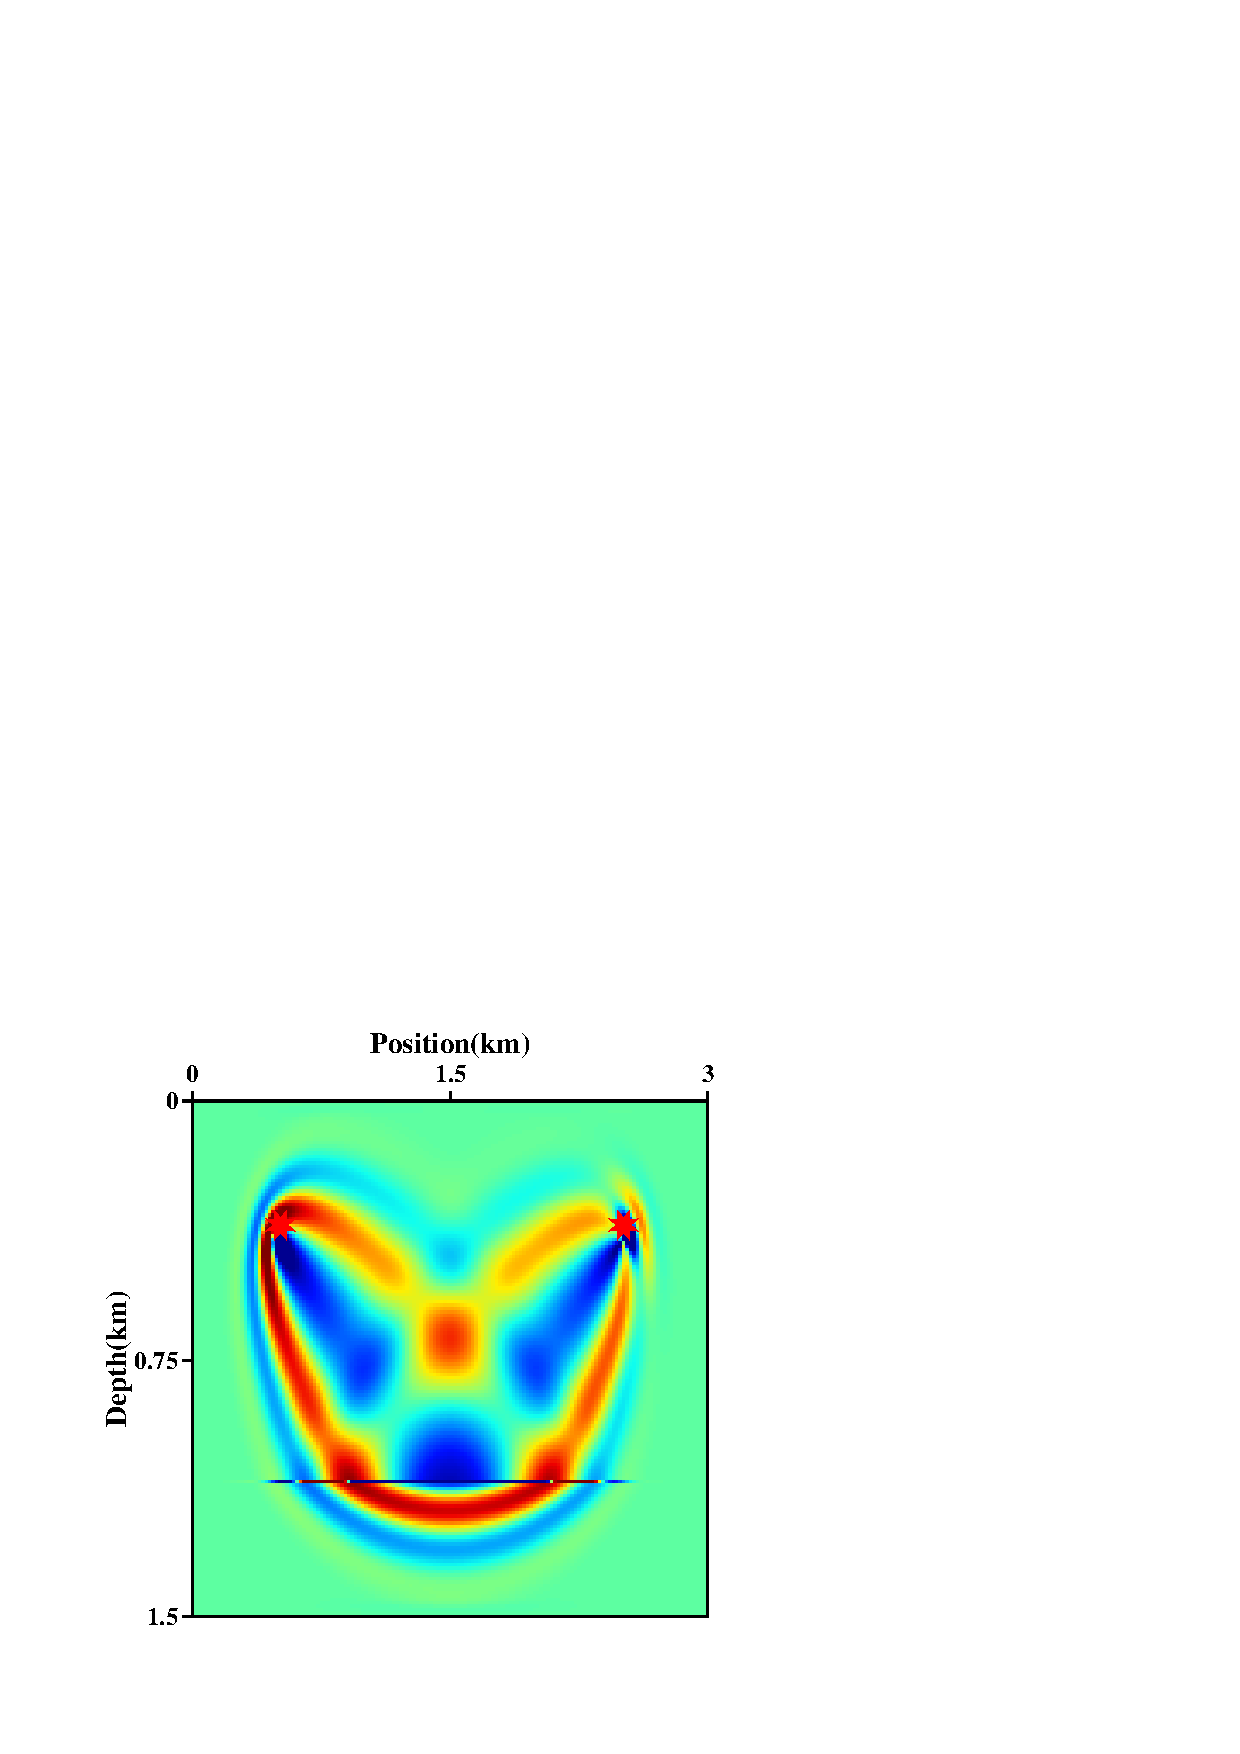
\includegraphics[width=0.25\textwidth]{Kernel/Vponlyvp.pdf}}
   \subfloat[]{\includegraphics[width=0.25\textwidth]{Kernel/Vsonlyvp.pdf}}\\
   \caption{Kernels with single reflector in $V_p$ model. (a) $V_p$ model, (b) $V_s$ model, (c) $K_{V_p}$, (d) $K_{V_s}$.}
   \label{fig:kernel1_vp}
\end{figure}

In the second model, we use the $V_s$ reflector (Fig \ref{fig:kernel2}a and b) to generate both PP
and PS reflection.
%The $V_s$ reflector produces both PP and PS data. 
The $V_p$ kernel excludes S-wavefield automatically because of the divergence operator 
implied in the term $\delta_{ij}\delta_{kl}$ (equation \eqref{eq:GradientVel}). 
However, $\delta \boldsymbol{\psi}$ contains the non-physical converted SP wavefields 
generated by the back-propagated  $\boldsymbol{\psi}^S$ at the location of reflector.
These SP wavefields make the $V_p$ kernel slightly different from that in Figure \ref{fig:kernel1_vp}c.
If we only back-propagate the PP data, $V_p$ kernel will be the same as Figure \ref{fig:kernel1_vp}c.

For $V_s$ kernel (Figure \ref{fig:kernel2}d), due to mode conversions, multi-wavepaths overlapping with each other 
make it much more complicated and difficult to find the correct PS reflection kernel. 
The straightforward utilization of this kernel in gradient calculation will very likely cause severe
cross-talk during reflection inversion.
According to equation
\eqref{eq:decompkernel}, we calculate the components of $K_{V_s}$, as shown in Figure
\ref{fig:kernel2_vs_decomp}. The $K^{PP}_{V_s}$ is similar to $K^{PP}_{V_p}$ but with an opposite
sign. $K^{PS}_{V_s}$ and $K^{SP}_{V_s}$ mainly consist of high-wavenumber energy, which in fact are
the migration impulse of cross-mode wavefields. Most importantly, 
we expect to update the $V_s$ model through the S-wavepath in PS reflection, while
$K^{SS}_{V_s}$ (Figure 3\ref{fig:kernel2_vs_decomp}d) is exactly what we want.
%S-wave part of the PS reflection wavepath. 
Therefore, we recommend using $K^{SS}_{V_s}$ to mitigate the cross-talks in $V_s$ gradient calculation.


\begin{figure}[!htb]
   \centering
   \subfloat[]{\includegraphics[width=0.250\textwidth]{Kernel/2vp.pdf}}
   \subfloat[]{\includegraphics[width=0.250\textwidth]{Kernel/2vs.pdf}}\\
   \subfloat[]{\includegraphics[width=0.250\textwidth]{Kernel/Vponlyvs.pdf}}
   \subfloat[]{\includegraphics[width=0.250\textwidth]{Kernel/Vsonlyvs.pdf}}\\
   \caption{Kernels with single reflector in $V_s$ model. (a) $V_p$ model, (b) $V_s$ model, (c) $K_{V_p}$, (d) $K_{V_s}$.}
   \label{fig:kernel2}
\end{figure}

\begin{figure}[!htb]
   \centering
   \subfloat[]{\includegraphics[width=0.250\textwidth]{Kernel/VsonlyvsPP.pdf}}
   \subfloat[]{\includegraphics[width=0.250\textwidth]{Kernel/VsonlyvsPS.pdf}}\\
   \subfloat[]{\includegraphics[width=0.250\textwidth]{Kernel/VsonlyvsSP.pdf}}
   \subfloat[]{\includegraphics[width=0.250\textwidth]{Kernel/VsonlyvsSS.pdf}}
   \caption{Four components of $K_{V_s}$. (a) $K_{V_s}^{PP}$, (b) $K_{V_s}^{PS}$, (c) $K_{V_s}^{SP}$, (d) $K_{V_s}^{SS}$.}
   \label{fig:kernel2_vs_decomp}
\end{figure}
\subsection{Workflow of elastic WERTI}
DIW extracts the reflection traveltime differences in data domain. In elastic case, %PP and PS reflections 
the cross points between different mode-conversions would be singularities for DIW.
%In elastic case, it is common to observe that different mode-conversions, mainly PP
%and P-S events, overlap and intersect with each other. The cross points between events
%would be singularities for traveltime difference estimation through DIW.
Therefore, $\tau(\mathbf{x_r},t;\mathbf{x_s})$ would be inaccurate if using the
original multicomponent seismic data, which makes equation \eqref{eq:GradientVel} difficult to implement.
Besides, according to the reflection kernel analysis, individually injecting PP or PS recordings also 
can mitigate the cross-talk in gradient calculation. 
Thus, we decompose the observed and calculated data into P- and S-wave
parts through P/S separation  of multi-component seismograms \cite[]{Li2016a}.
%Then we can easily get the separated vector P and S-wave seismograms for each shot.
In this way, the traveltime differences can be decoupled into P- and
S-wave part, with which we can implement the elastic WERTI through a two-stage
workflow, i.e. the P-wave stage followed by the S-wave stage.

In the first stage, we use PP traveltime to recover $V_p$ model. 
%The perturbation of $V_p$ ($\delta V_p$) through  elastic reverse time
%migration (ERTM). 
Since only the traveltime is considered in WERTI, 
just ERTM is applied to obtain the image rather than in a least-square manner (LSRTM) to find the correct reflectivity. 
Therefore, the objective function is:
\begin{equation}
	E_{pp}=\frac{1}{2}\int\tau^2_{pp}(\mathbf{x_r},t;\mathbf{x_s})dtd\mathbf{x_r}d\mathbf{x_s}.
    \label{eq:ObjectivefunctionPP} 
\end{equation}
Thus, we can obtain the gradient of  $V_p$ ($\frac{\partial E}{\partial
V_p}$), just using the P-wave seismograms to
calculate RHS of equation \eqref{eq:AdjointWE} and replacing $\delta c_{ijkl}$ with
$\delta V_p$ in equation \eqref{eq:DeltaWE} and \eqref{eq:AdjointDeltaWE}.

In the S-wave stage, 
%a similar strategy is applied using the P-S reflection
%traveltime. 
the objective function becomes:
\begin{equation}
	E_{ps}=\frac{1}{2}\int\tau^2_{ps}(\mathbf{x_r},t;\mathbf{x_s})dtd\mathbf{x_r}d\mathbf{x_s}.
    \label{eq:ObjectivefunctionPS} 
\end{equation}
However, the implementation is a little different from the previous stage. After the
P-wave stage inversion, the background $V_p$ should be well recovered. As we know, in
most cases $V_p$ and $V_s$ share the same structure in the subsurface. Therefore, we
recommend to use the well imaged $\delta V_p$ instead of $\delta V_s$ to generate the PS reflections. 
Besides, in order to make sure that reflected S-wavepath is used to update $V_s$, wave mode decomposition 
is implemented to calculate $K^{SS}_{V_s}$ with:
%we drop the first term in the RHS of equation \eqref{eq:GradientCijkl} when
%calculating $\frac{\partial E}{\partial V_s}$. And also wave mode decomposition is
%applied to make sure that only S-wave energy are involved:
\begin{equation}
	\frac{\partial E_{ps}}{\partial V_s}=-2\rho V_s
	\int (\frac{\partial \delta u^S_{i}}{\partial
    x_j}\frac{\partial \psi^S_{k}}{\partial x_l})
	(\delta_{ik}\delta_{jl}+
	\delta_{il}\delta_{jk}).
    \label{eq:GradientVel_MD}
\end{equation}
This is similar to the gradient precondtioning for EFWI proposed by \cite{WangEtAl2017}. The mode
decomposition can mitigate parameter trade-offs and suppress artifacts for the
$V_s$ inversion.
\begin{figure}[!htb]
   \centering
   \subfloat{\includegraphics[width=0.25\textwidth]{sigbee2/Fig/cuttruevp.pdf}}
   \subfloat{\includegraphics[width=0.25\textwidth]{sigbee2/Fig/cuttruevs.pdf}}\\
   \subfloat{\includegraphics[width=0.25\textwidth]{sigbee2/Fig/cutinitvp.pdf}}
   \subfloat{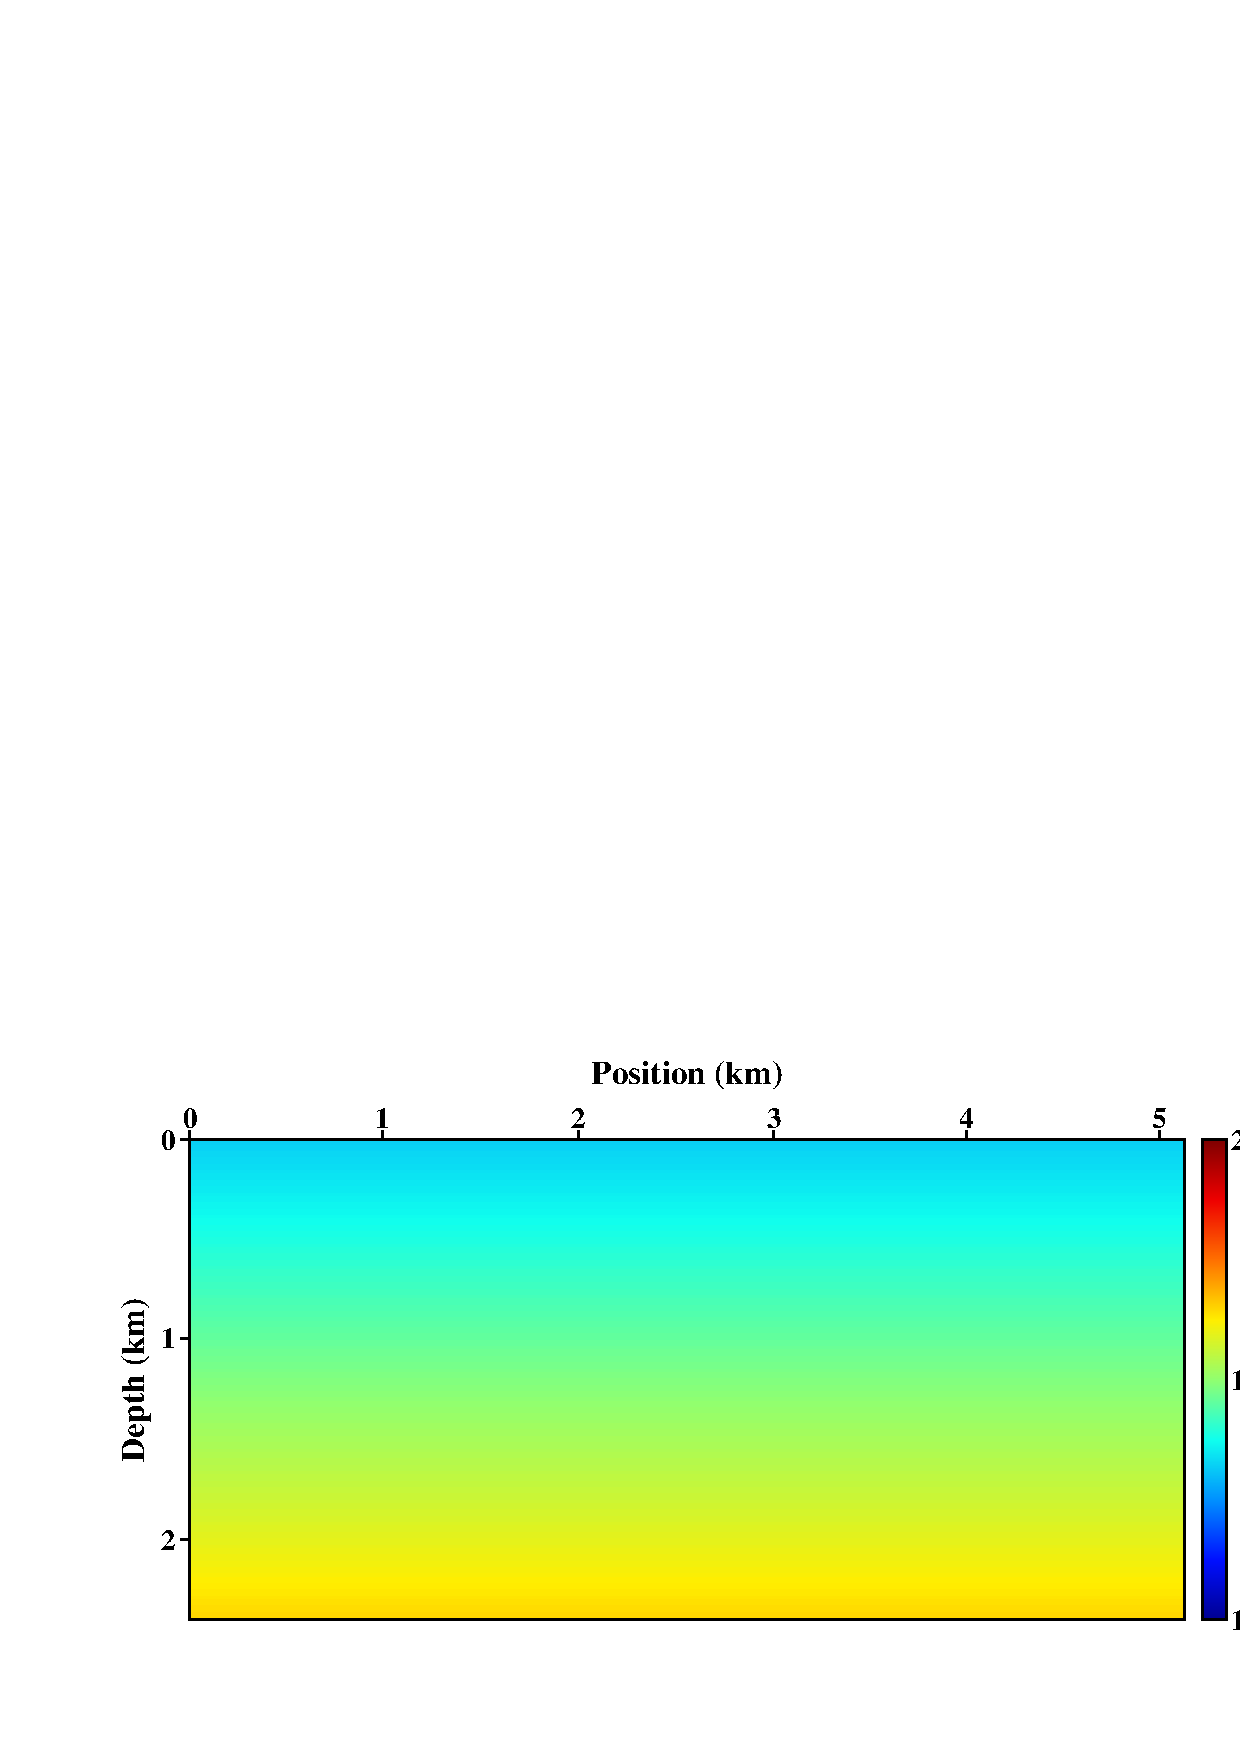
\includegraphics[width=0.25\textwidth]{sigbee2/Fig/cutinitvs.pdf}}
   \caption{Sigbee2A model example. On the top are true models of 
   $V_p$ (a) and $V_s$ (b). On the bottom are initial models of $V_p$ (c) and $V_s$
   (d) linearly increasing with depth. }
   \label{fig:TrueAndInitial}
\end{figure}

\section{numerical example}
We select a part of the Sigsbee2A model (Figure
\ref{fig:TrueAndInitial}a and \ref{fig:TrueAndInitial}b) to test the inversion algorithm and strategy.
The $V_s$ model is generated using fixed Poisson's ratio. 
The initial model for E-WERTI are shown in 
Figure \ref{fig:TrueAndInitial}c and \ref{fig:TrueAndInitial}d.
%show the initial model of
%$V_p$ and $V_s$, which linearly increase with depth. 
%We can see 
The linearly increasing initial model of $V_p$ is generally lower while 
$V_s$ is higher than the true model, and both of
them are far from the true value. 36 shots are evenly deployed on the surface and receivers are
fixed with a maximum offset of 4km. 
The main frequency of P-wave source is 15Hz.
%Pure P-wave source is used with a main frequency of 15Hz.

Figure \ref{fig:InvertedModel}a and \ref{fig:InvertedModel}b show the inverted results of E-WERTI.
%Since the linearly increased initial model is quite far from the true value, certainly there will be
%cycle-skipping problem if we use this for conventional EFWI. However, 
After
40 iterations for each stage, WERTI provides a good recovery of the background
information for both $V_p$ and $V_s$. 
Nonetheless, on the right part, the reflection coverage of surface observation is insufficient for
WERTI to rebuild the long-wavelength components. 
Using the inverted results of WERTI as starting
models, we also perform the conventional EFWI. As shown in Figure \ref{fig:InvertedModel}c and
\ref{fig:InvertedModel}d, both of the inverted $V_p$ and $V_s$ models are well
reconstructed except the right part.
\section{Conclusions}
Reflection traveltime inversion only minimizes traveltime misfits which are more sensitive
and linearly related to the low-wavenumber model perturbation. 
The kernel analysis of different wave modes show that mode decomposition can 
suppress artifacts and recover the correct reflection wavepath in gradient calculation.
With the aid of DIW and
P/S separation of 3C seismograms, we can obtain the travel time differences of PP and PS
reflections, respectively. 
To build the long-wavelength component of the model, we introduce a two-stage WERTI
workflow by firstly using PP then PS reflections, through which the nonlinearity of reflection
inversion is reduced effectively. 
In the second stage, the wave mode
decomposition is introduced to calculate the gradient of $V_s$ to mitigate the trade-off between
$V_p$ and $V_s$.
The Sigsbee2A model example shows that even starting with a bad initial model, the
two-stage E-WERTI can provide reliable starting model for conventional EFWI. 

\begin{figure}[!htb]
   \centering
   \subfloat[]{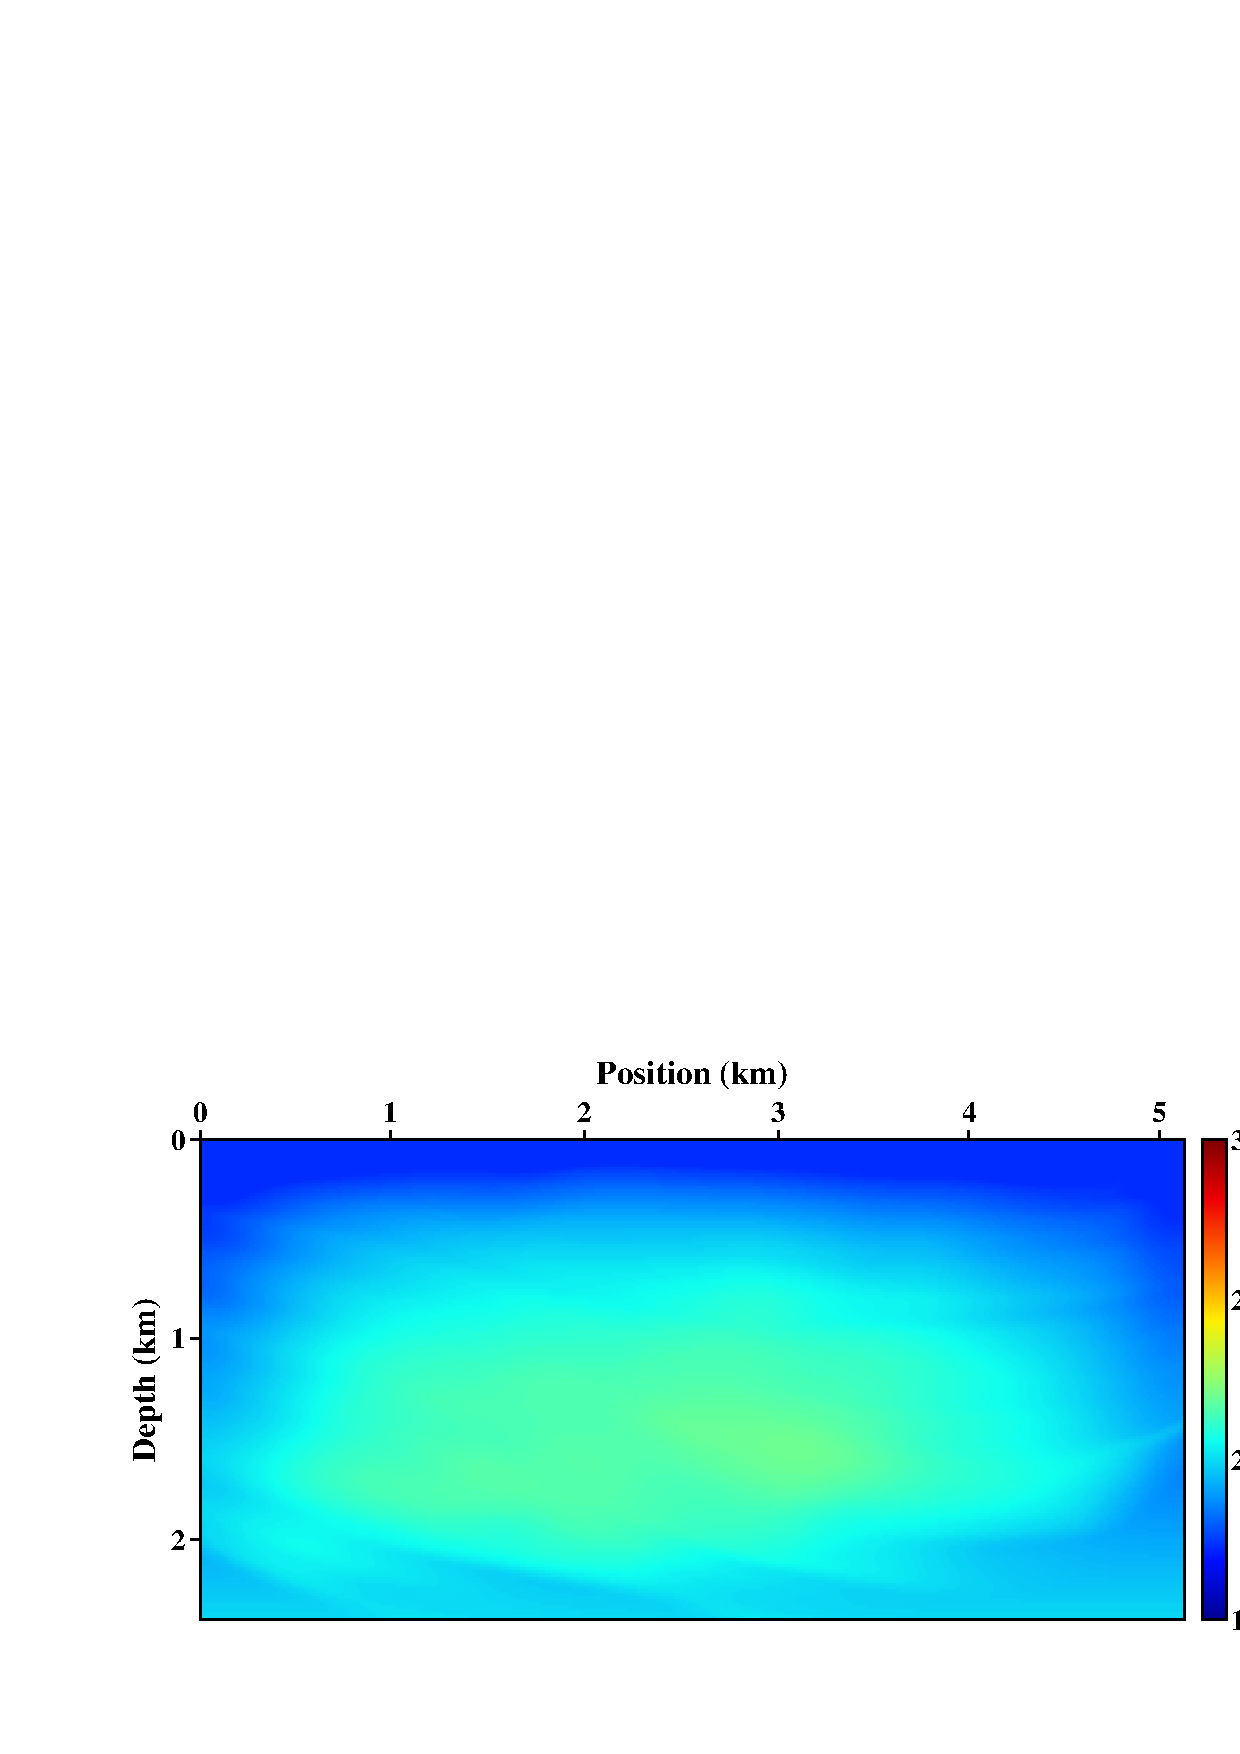
\includegraphics[width=0.38\textwidth]{sigbee2/Fig/newinit3vp.pdf}}\\
   \subfloat[]{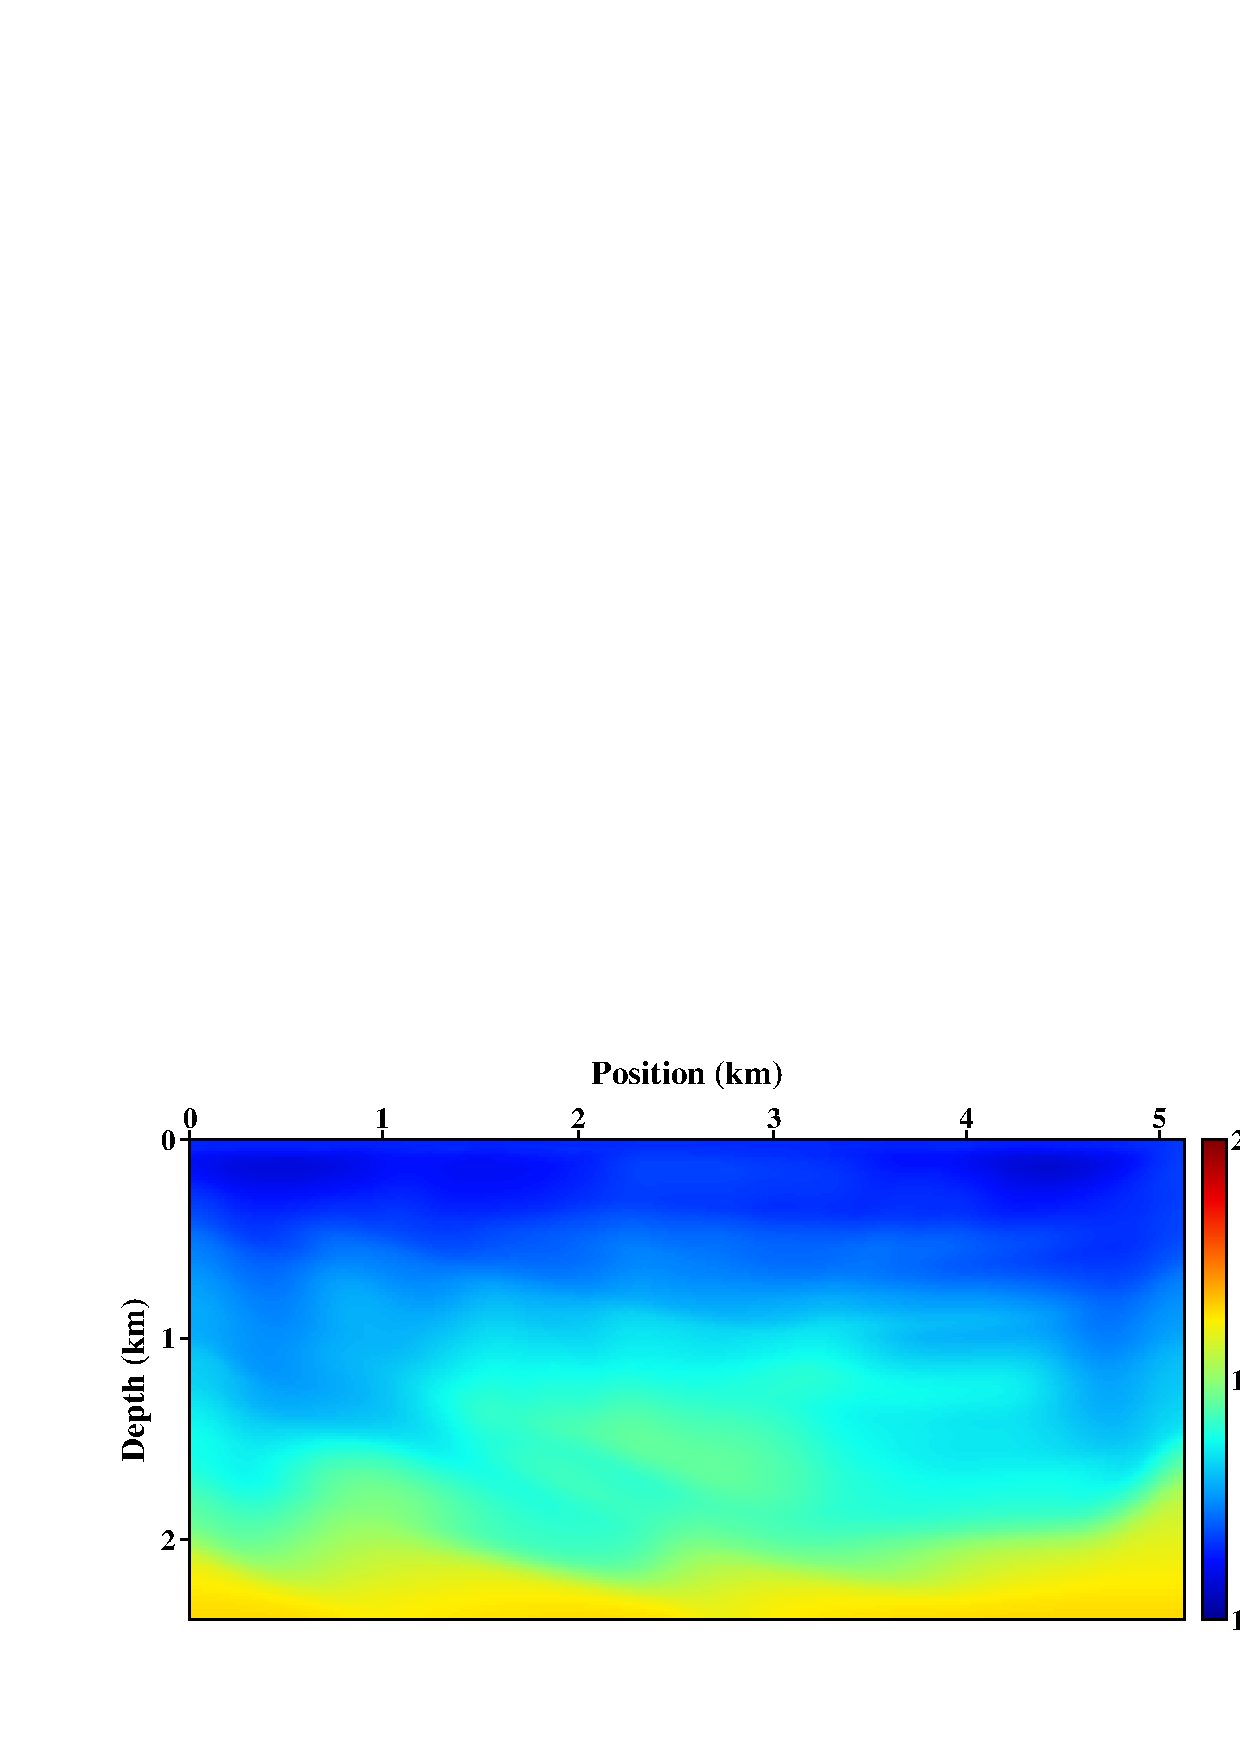
\includegraphics[width=0.38\textwidth]{sigbee2/Fig/newinit3vs.pdf}}\\
   \subfloat[]{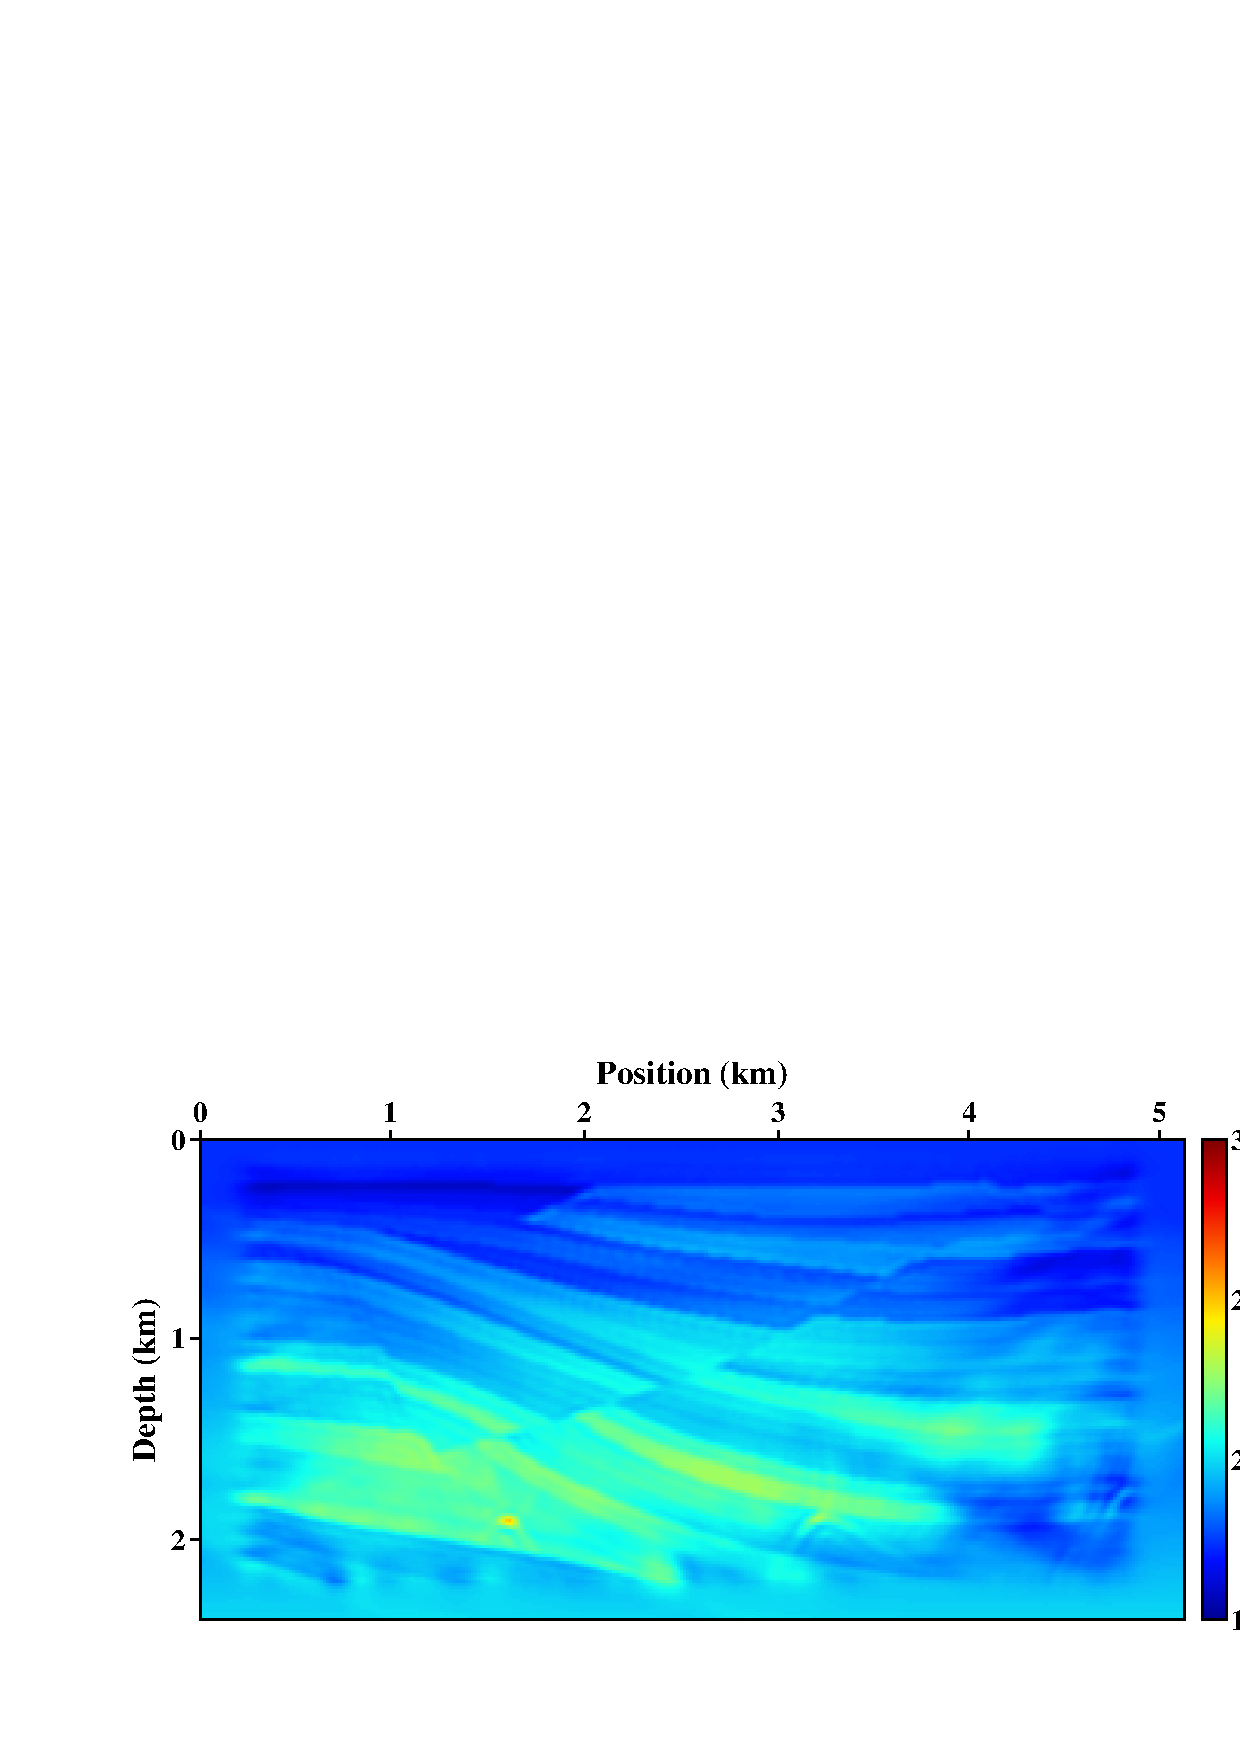
\includegraphics[width=0.38\textwidth]{sigbee2/Fig/nodevp.pdf}}\\
   \subfloat[]{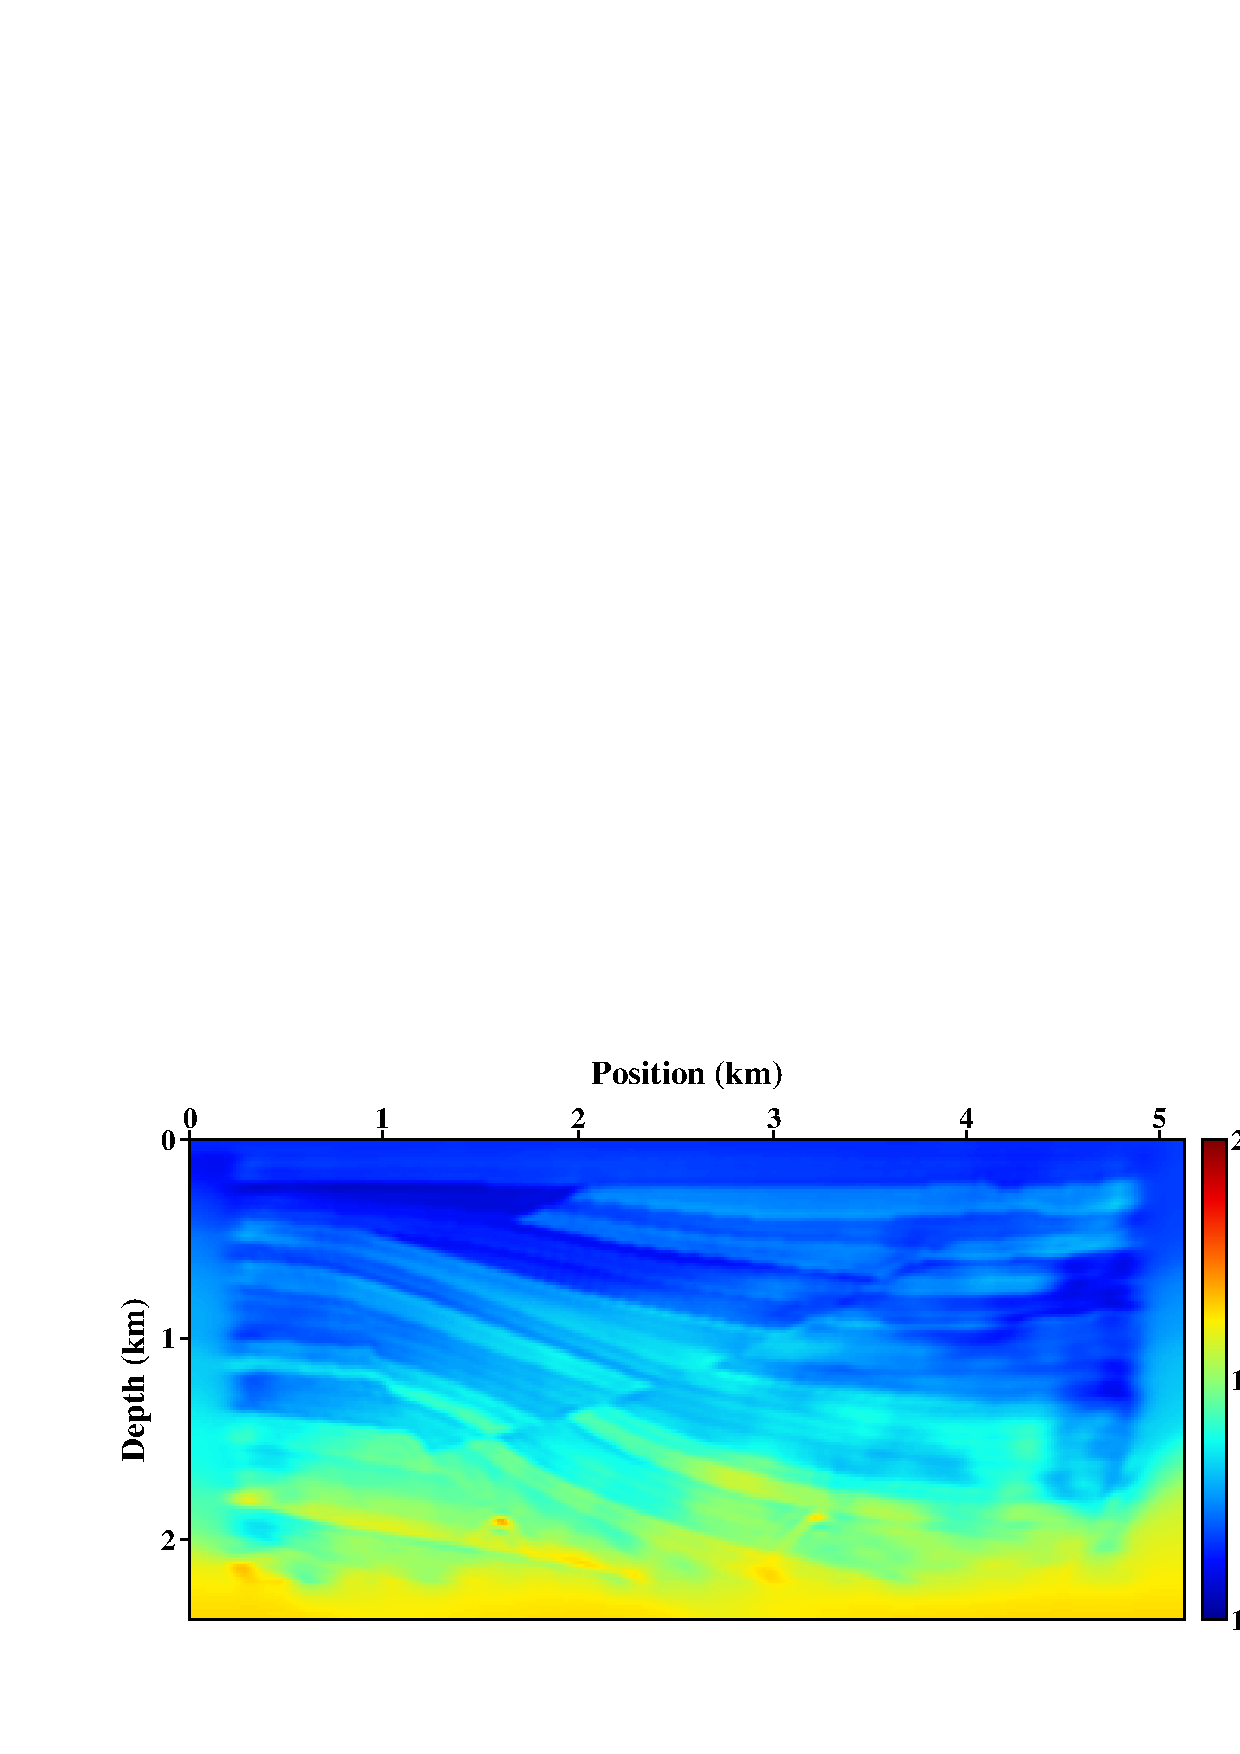
\includegraphics[width=0.38\textwidth]{sigbee2/Fig/nodevs.pdf}}
   \caption{Inverted results of WERTI and EFWI. (a) and (b) are inverted $V_p$ and
	   $V_s$ model through two-stage elastic WERTI with the linearly increased models
	   as initial models. (c) and (d) are inverted $V_p$ and $V_s$ through EFWI using
   (a) and (b) as starting models.}
   \label{fig:InvertedModel}
\end{figure}
\section{Acknowledgement}
This work is supported by the
National Natural Science Foundation of China (NO.41474099, 41674117 \& 41630964). 
This paper is also based upon the work supported by the King Abdullah University of Science
and Technology (KAUST) Office of Sponsored Research (OSR) under award NO. 2230.
We appreciate the open-source package of DENISE from
\textit{https://github.com/daniel-koehn/} and Mines Java Toolkit from
\textit{https://github.com/dhale}.
We thank the useful advice from Tariq Alkhalifah (KAUST), Qiang Guo (KAUST), Zedong Wu (KAUST),
Chenlong Wang (Tongji University) and Benxin Chi (Los Alamos).



